\section{Evaluation}
\label{sec:casestudy}
In this section, we evaluate \AVOIRmethodname{}.variants through three real-world case studies.
Direct comparisons with existing work are impossible since no other work (to our knowledge) facilitates a general-purpose inference engine for online fairness auditing using arbitrary measures.
We can, however, implement VF's~\cite{bastani2019probabilistic} inference rules within \AVOIRmethodname{} (denoted as \AVOIRmethodname{}-VF).
Note that \AVOIRmethodname{}-VF sidesteps the assumptions of having a known data-generating distribution (made possible by \AVOIRmethodname{}'s reliance on confidence sets), making this variation a more practical and efficient algorithm. 
We denote \AVOIRmethodname{}-OB as the implementation that utilizes the abovementioned optimizations. 
Across the studies, the role of chosen threshold probabilities is similar to that of p-values in statistics.
Typical p-values tend to be $0.05$ and $0.1$, which we demonstrate in the RateMyProfs and COMPAS risk assessment study. 
In our case study of prior work~\cite{angwin2016machine}, we stick to the available definitions and thresholds used in the original analysis.
We expect that regulators will set the threshold probabilities on a case-by-case basis, e.g,, $0.15$ for illustration purposes in the adult income study.%, and we provide the adult income study with  $\Delta =0.15$ as an example.

%An important case study on the COMPAS dataset can be found in Appendix~\ref{sec:appendix:additional-case-studies}. 
\subsection{Rate My Profs}
\label{sec:casestudy:rmp}
\begin{figure}
    \centering
    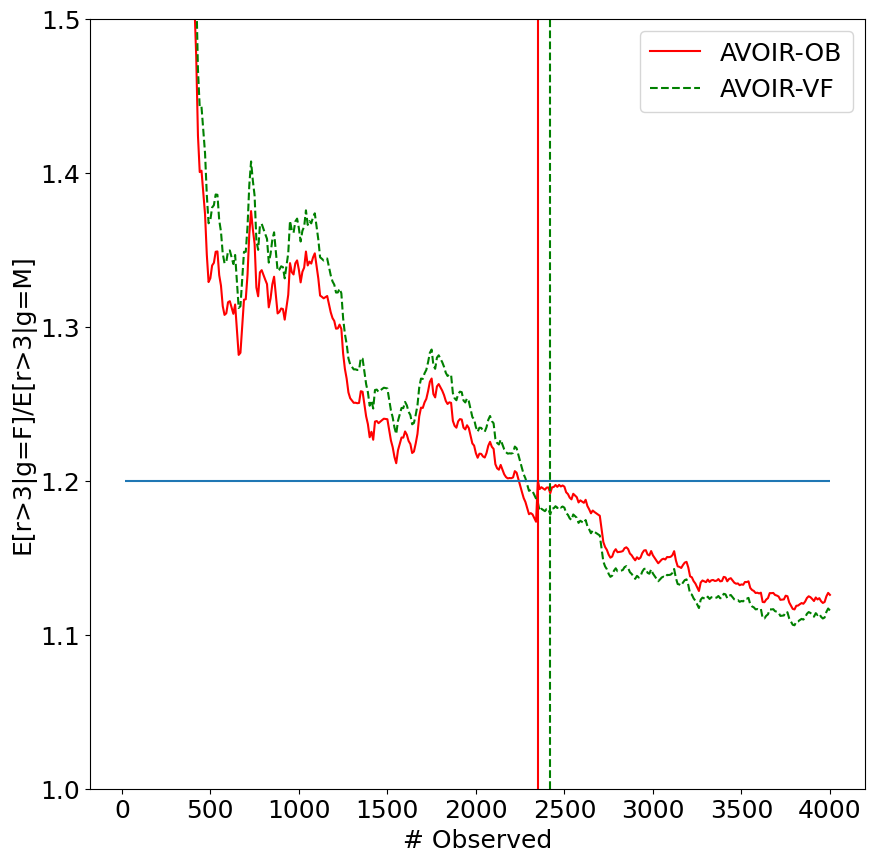
\includegraphics[width=0.5\linewidth,alt={Line plot showing the upper bound of the first half of a gender fairness specification for the RateMyProfs dataset. Our optimized \AVOIRmethodname{}-OB achieves the bound using fewer samples.}]{avoir/images/ratemyprofs.png}
    \caption{Bounds for first half of a gender-fairness specification generated by \AVOIRmethodname{}-OB and \AVOIRmethodname{}-VF for \textit{RateMyProfs}, a real-world dataset. Vertical lines show the step at which the methods can provide a guarantee of failure for the upper bounds with $\Delta <= 0.05$. Blue horizontal line represents the constant term in the inequality.}
    \label{fig:casestudy:rmp}
\end{figure}
This section provides a detailed black-box machine learning model-based case study on a real-world dataset.
This case study uses the Rate My Professors (RMP) dataset~\cite{keymanesh2021fairness}. 
This dataset includes professor names and reviews for them written by students in their classes, ratings, and certain self-reported attributes of the reviewer.
Ratings are provided on a five-point scale (1-5 stars).
We use the preprocessing described in~\cite{keymanesh2021fairness} to infer the gender attribute for the professors.
This dataset is divided into an 80-20 split (train-test).
We then train a BERT-based transformer model~\cite{devlin2019bert} on the training split.
We use the implementation from the simpletransformers\footnote{https://simpletransformers.ai/} package.
The loss function chosen is the mean-squared error from the true ratings.
On the test set, we track a gender-fairness specification in the model outputs:
\begin{lstlisting}[columns=flexible, language=Python, basicstyle=\small]
(E[r > 3 | gender = F] / E[r > 3 | gender = M < 1.2) & 
(E[r > 3 | gender = M)] / E[r > 3 | gender = F] > 0.8)
\end{lstlisting}
We set the failure probability $\Delta = 0.05$. 
\texttt{OPT} is run after each batch (5 items/batch).
Figure~\ref{fig:casestudy:rmp} shows that \AVOIRmethodname{}-OB\footnote{OB = Optimized Bounds} can provide a guarantee in $\mathbf{2.5\%}$ fewer iterations than \AVOIRmethodname{}-VF. 
Note also that the OB guarantee provided tries to optimize for the failure probability while staying under the required threshold, remaining closer to the required threshold in subsequent steps.

\subsection{Adult Income}
\label{sec:casestudy:adult}
In this case study, we analyze the Adult income dataset~\citep{kohavi1996scaling}.
The historical dataset labels individuals from the 1994 census as having a \emph{high-income} ($>50$k a year) or not ($\leq50$k a year).
We consider this column of data as a black-box measurement. 
US Federal laws mandate against race and sex-based discrimination.
Thus, the specification we start our analysis with is a group fairness property for federal employees that monitors the difference of the proportions of individuals with sex marked male vs. female with a high income should be less than $0.5$.
In addition, we ensure that the difference between individuals with race marked white and non-white should have a difference of less than $0.5$.  
Thus, we use an \textit{intersectional} fairness criterion.
The associated specification is given below, where \texttt{h} is an indicator for whether an individual is \emph{high-income} is the binary classification output of our model:

\begin{lstlisting}[columns=flexible, language=Python, basicstyle=\small]
   (E[h | sex=M] - E[h | sex=F] < 0.5) & \ 
   (E[h | race=W] - E[h | race!=W] < 0.5)
\end{lstlisting}

In this example, we set the failure threshold probability $\Delta = 0.15$
\begin{figure}
    \centering
    \begin{subfigure}{0.6\linewidth}
    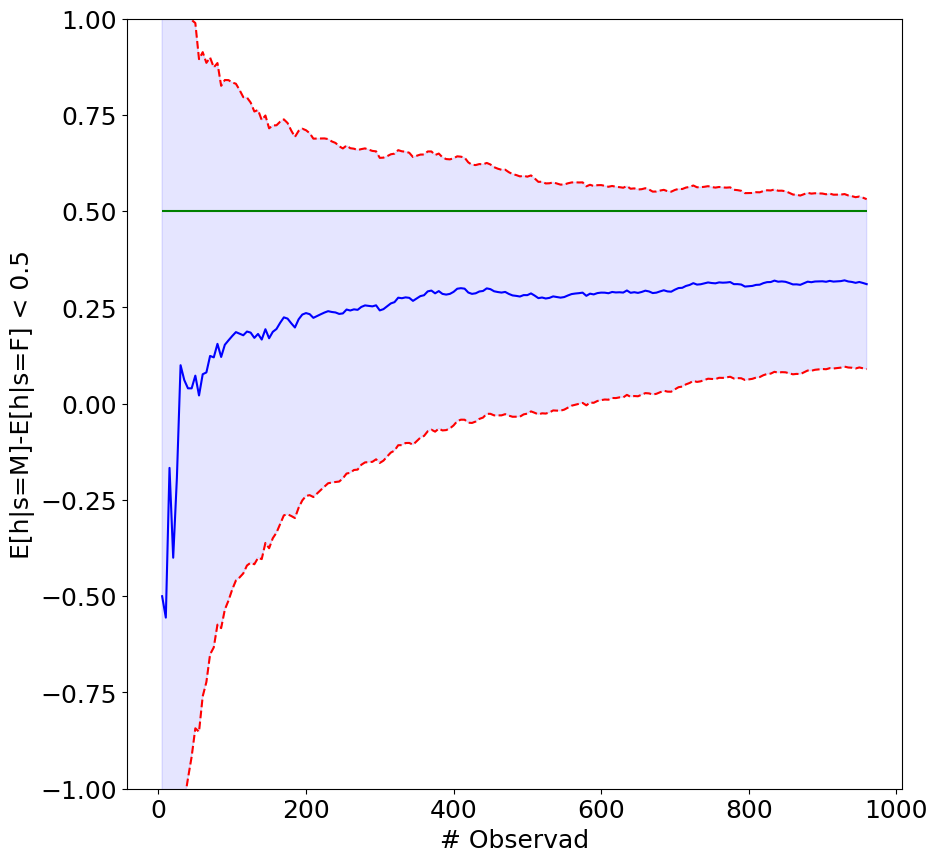
\includegraphics[width=\linewidth,alt={Confidence interval line plots showing group fainess differences for sex.}]{avoir/images/adult-left-initial.png}
    \caption{Group fairness for sex. Difference in ratio of high income (left subexpression).}
    \label{fig:casestudy:adult:specplot:left}
    \end{subfigure}
    %
    \begin{subfigure}{0.6\linewidth}
    \centering
    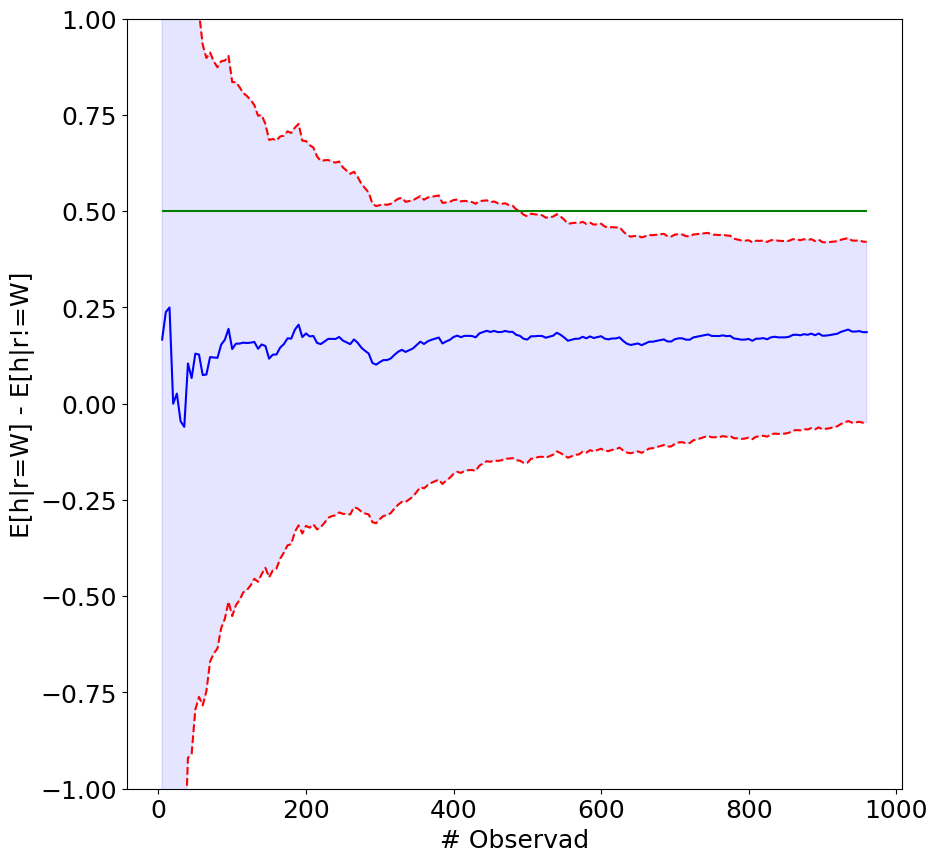
\includegraphics[width=\linewidth,alt={Confidence interval line plots showing group fairness for race.}]{avoir/images/adult-right-initial.png}
    \caption{Group fairness for race. Difference in ratio of high-income earners (right subexpression). }
    \label{fig:casestudy:adult:specplot:right}
    \end{subfigure}
    \caption{\figtop{} Red dotted lines, the upper bounds of the value cannot be guaranteed to be under the threshold at the specified failure probability. \figbottom{} Guarantee possible with given data. Green lines represent the constant term, and dark blue is the empirical mean.}
\end{figure}
When run with this specification, the generated bounds cannot be achieved with the available data. 
We can then use the iterative refinement associated with subexpressions to analyze different components of the specification. 
The plot corresponding to the left subexpression is shown in Figure~\ref{fig:casestudy:adult:specplot:left} shows that guarantees cannot converge under the threshold with the given number of data samples. 
An auditor can now choose to either reduce the guarantee (i.e. increase $\Delta$) or increase the threshold. 
Next, analyzing the right subexpression, the race group fairness term can be guaranteed to be under the threshold (Figure~\ref{fig:casestudy:adult:specplot:right}).
Using this information, an auditor can make a decision to increase the threshold on the group fairness term for sex. 
As a hypothetical, suppose they increase it from $0.5$ to $0.55$ and rerun the analysis.
OB can provide a guarantee at this threshold within 870 steps, whereas VF can provide it at 960 steps, demonstrating a relative improvement of about $\mathbf{10.35\%}$.
Additionally, the optimal $\Delta$ split across the terms is $\approx (0.135, 0.36 * 10^4)$, which is far from the equal split allocated by VF.
The reason for this split is that increasing the threshold for the first time provides the optimizer with additional legroom to better distribute the failure probabilities between the two terms.

\subsection{COMPAS Risk Assessment}

The Correctional Offender Management Profiling for
Alternative Sanctions (COMPAS) recidivism risk score data is a popular dataset for assessing machine bias of commercial tools used to assess a criminal defendant's likelihood to re-offend.
The data is based on recidivism (re-offending) scores derived from software released by Northpointe and widely used across the United States for making sentencing decisions.
In 2016, \citet{angwin2016machine} at ProPublica released an article and associated analysis code critiquing machine bias associated with race present in the COMPAS risk scores for a set of arrested individuals in Broward County, Florida, over two years.
The analysis concluded that there were significant differences in the risk assessments of African-American and Caucasian individuals.
Northpointe pushed back in a report~\citep{dieterich2016compas} firmly rejecting the claims made by the ProPublica article; instead, they claimed that \citet{angwin2016machine} made several statistical and technical errors in the report.
In this case study, we use \AVOIRmethodname{} to study the claims of the two reports mentioned above. 
%First, we start with the data released by ProPublica and load it into a pandas-simulated DB.
We create a materialized view of the ProPublica dataset by reproducing the preprocessing steps in the publicly available ProPublica analysis  notebook\footnote{https://github.com/propublica/compas-analysis}.
We look at ``Sample A''~\citep{dieterich2016compas}, where the analysis of the ``not low'' risk assessments using a logistic regression model reveals a high coefficient associated with the factor associated with race being African-American.
In terms of a fairness metric, this corresponds to false positive rate (FPR) balance (predictive equality)~\citep{verma2018fairness} metrics. 
The associated specification in \AVOIRmethodname{} grammar would be

\begin{lstlisting}[columns=flexible, language=Python, basicstyle=\small]
   E[hrisk | race=African-American & recid=0] / 
   E[hrisk | race=Caucasian & recid=0] < 1.1
\end{lstlisting}

Where \verb|hrisk| is an indicator for high-risk assessments made by the \emph{black-box} COMPAS tool as defined by ~\citet{angwin2016machine},  \verb|recid| is an indicator for re-offending within two years of first arrest, and a $90\%$-rule is used as the threshold. 
We choose a failure threshold probability of $\Delta = 0.1$, with the optimization run after every batch of $5$ samples.
\AVOIRmethodname{} finds that when the decisions are made sequentially, online, the assertion for specification violation cannot be made with the required failure guarantee.

By analyzing the component subexpressions, one can glean that \AVOIRmethodname{} cannot optimize since the lower FPR in the denominator (FPR for Caucasian individuals) increases the overall variance and limits the ability to optimize for guarantees. 
We follow this analysis by using the reciprocal specification, i.e.,
\begin{lstlisting}[columns=flexible, language=Python, basicstyle=\small]
   E[hrisk | race=Caucasian & recid=0] /
   E[hrisk | race=African-American & recid=0] > 0.9
\end{lstlisting}

We find that the specification is guaranteed to be violated with a confidence of over $1 - \Delta = 0.9$ probability, and \AVOIRmethodname{} can detect this violation within about half the number of available assessments (3350 steps) when run in an online setting.
Figure~\ref{fig:casestudy:compas:propublica} demonstrates the progression of the tracked expectation term. 
Thus, if deployed with the corrected specification, \AVOIRmethodname{} would be able to alert Northpointe/an auditor of a violation/potentially-biased decision-making tool.

\begin{figure}
    \centering
    \begin{subfigure}{0.6\linewidth}
        \centering
        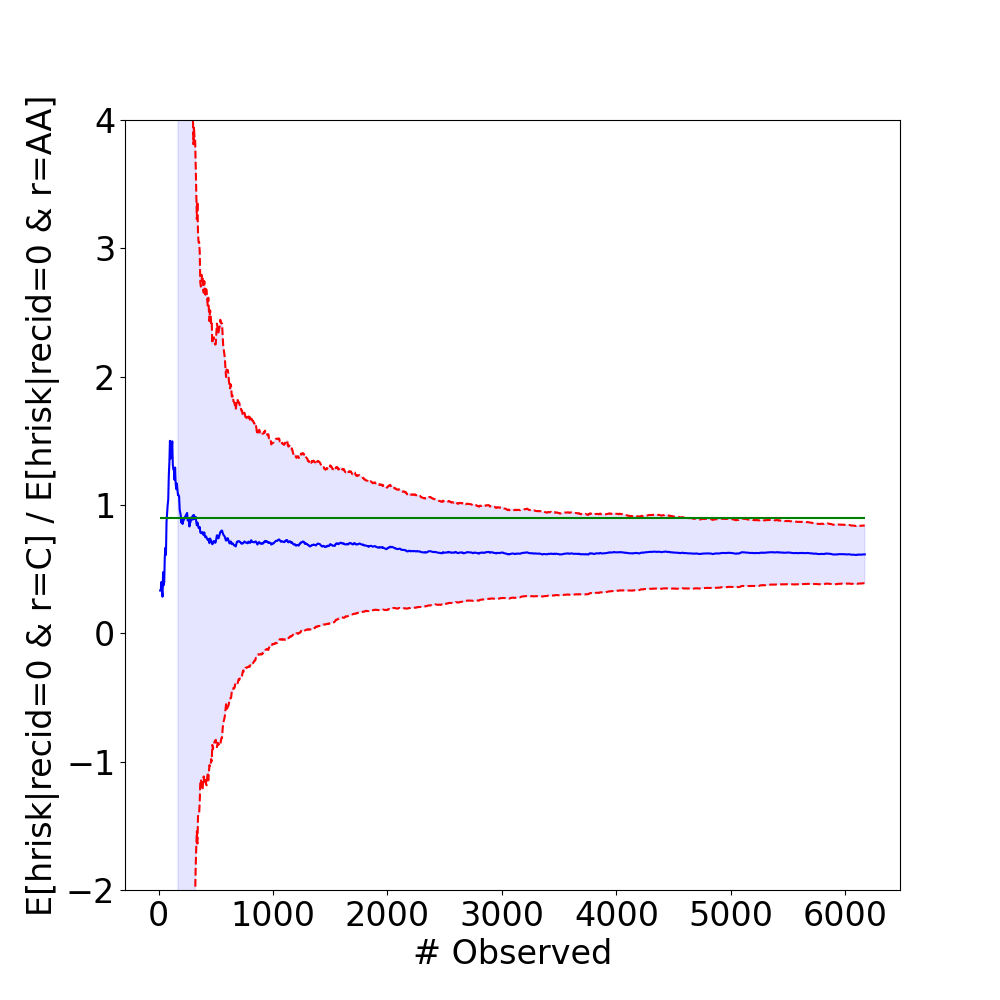
\includegraphics[width=0.8\linewidth,alt={Confidence line plots showing that the claims made by Propublica reach the required uncertainty threshold with the available samples.}]{avoir/images/compas-propublica-et.png}
        \caption{(ProPublica) COMPAS, ``Sample A'' False Positive Rate Bias specification required to \emph{above} the $10\% \implies 0.9$ threshold converges to a value that can be guaranteed to be \emph{under} the required threshold.}
        \label{fig:casestudy:compas:propublica}
    \end{subfigure} 
    %
    \begin{subfigure}{0.6\linewidth}
        \centering
        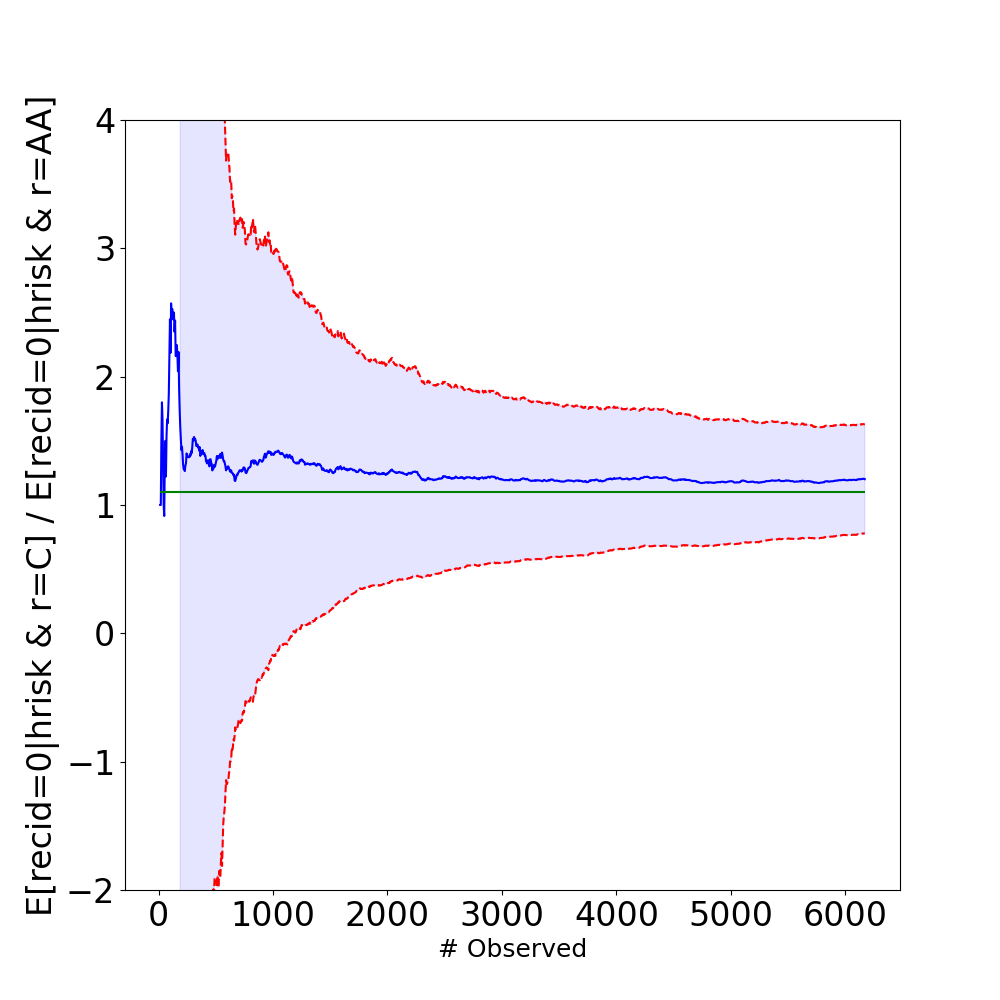
\includegraphics[width=0.8\linewidth,alt={Confidence line plots showing that the claims made by Northpointe do not reach the required uncertainty threshold with the available samples}]{avoir/images/compas-northpointe-et.png}
        \caption{(Northpointe) ``Sample B'' analysis done by Northpointe using False Discovery Rate that opposed the ProPublica reports.}
        \label{fig:casestudy:compas:northpointe}
    \end{subfigure}
    \caption{COMPAS dataset case study.}
\end{figure}


The Northpointe report~\citep{dieterich2016compas} makes several claims about the shortcomings of this analysis.
One of the primary claims is that \citet{angwin2016machine} used an analysis based on ``Model Errors'' rather than ``Target Population Errors''.
In fairness specification terms, this refers to the difference between a False Positive Rate (FPR) balance vs. False Discovery Rate (FDR) balance, i.e., balancing for predictive parity over predictive equality. 
In probabilistic terms, the difference amounts to comparing $\Pr[\hat{Y} = 1 | Y = 0, g=1, 2]$ (FPR) vs $\Pr[Y = 0 | \hat{Y} = 1, g=1, 2]$ (FDR), where $\hat{Y}$ refers to the decision made by the algorithm, $Y$ refers to the true value, and $g = 1, 2$ reflects group membership~\citep{verma2018fairness}.
This analysis is run on the dataset subset dubbed ``Sample B''.
To test their hypothesis, we reproduce the corresponding preprocessing steps and run both versions (numerator and denominator being Caucasian) of the corresponding specification under the same setup as earlier. 
Despite the point estimate being within the required threshold, we find that neither version can be guaranteed with the required confidence in the given data.
Due to the paucity of space, we describe only one of the two variants with the corresponding figure (Figure~\ref{fig:casestudy:compas:northpointe}).
\begin{lstlisting}[columns=flexible, language=Python]
   E[recid=0 | race=Caucasian & hrisk] /
   E[recid=0 | race=African-American & hrisk] > 0.9
\end{lstlisting}


We note that the Northpointe report~\citep{dieterich2016compas} does not provide confidence intervals for their claim. 
Further, even though the report does not release associated code, the point estimates of the False Discovery Rates (FDRs) match those present in the report, which increases our confidence in our \AVOIRmethodname{}-based analysis. 

The back-and-forth exchange has been the subject of much discussion in academic and journalistic publications~\citep{feller2016computer, washington2018argue}.
Seminal work by \citet{kleinberg2017inherent} proved the impossibility of simultaneously guaranteeing certain combinations of fairness metrics.
While \AVOIRmethodname{} cannot circumvent this problem, its usage can help audit claimed guarantees on defined metrics.
We conclude this case study by noting that \AVOIRmethodname{} lends itself to successful analysis that is not possible with the VF implementation available online, which only provides support for a predefined set of specifications and requires access to a data-generating function.
In addition, we choose $0.1$ as the failure probability because it is one of the thresholds used in \cite{angwin2016machine}.  
We set it to the highest used threshold to allow leeway for the claim by Northpointe.
Even under this lax threshold, the analysis by Northpointe fails.